\section{Pianificazione}
Lo sviluppo del progetto viene organizzato e suddiviso nelle seguenti fasi:
\begin{itemize}
\item \textbf{Analisi preliminare};
\item \textbf{Progettazione Proof of Concept\textsubscript{g}};
\item \textbf{Codifica Proof of Concept\textsubscript{g}};
\item \textbf{Progettazione di dettaglio e codifica dei requisiti}.
\end{itemize}

%fase di Analisi preliminare

\subsection{Analisi preliminare}
Questo periodo comincia nel momento in cui vengono assegnati i capitolati e termina con l'inizio del periodo di Progettazione Proof of Concept\textsubscript{g}.\\
\begin{center}
\textbf{periodo:} dal 5-11-2022 al 14-12-2022\\
\end{center}
In questo periodo ci si concentra nel definire il way of working, creare tutta la documentazione necessaria e fare un analisi approfondita del capitolato scelto.  Questo periodo viene suddiviso nelle attività trattate nella seguente sezione.

\subsubsection{Attività}
\begin{itemize}
\item \textbf{\textit{Norme di Progetto}:} vengono individuati gli strumenti e le linee guida da seguire durante lo sviluppo del progetto;
\item \textbf{\textit{Piano di Progetto}:} documento in cui viene definita la pianificazione del progetto e le sue varie fasi,  in più fornisce un preventivo per ogni fase pianificata ed il totale costo ed ore necessario per la realizzazione del progetto;
\item \textbf{Analisi dei requisti:} viene eseguito uno studio approfondito dei requisti del capitolato scelto,  di conseguenza si costruisce un diagramma dei casi d'uso e un diagramma delle attività;
\item \textbf{\textit{Glossario}: } documento contenente la descrizione di termini di dominio del progetto, il \textit{Glossario} sarà continuamente aggiornato in base alla necessità.
\end{itemize}

\subsubsection{Periodi}
La fase di Analisi preliminare sarà suddivisa nei seguenti periodi:
\begin{itemize}
\item \textbf{Periodo 1:} \textit{dal 5-11-2022 al 16-11-2022},  pianificazione del periodo di Analisi preliminare,  suddivisone dei ruoli fra i componenti del gruppo,  prima stesura delle \textit{Norme di Progetto}, viene effettuata un'analisi dei rischi.  Inoltre ci sarà la continua stesura di verbali dopo ogni incontro con il gruppo e con il proponente\textsubscript{g};
\item \textbf{Periodo 2:} \textit{dal 16-11-2022 al 7-12-2022},  analisi dei requisti del capitolato scelto,  prima stesura del \textit{Glossario}, stesura del \textit{Piano di Progetto} con rispettivo preventivo della fase di Analisi preliminare.  I componenti del gruppo si impegnano a studiare le tecnologie necessarie per il compimento del progetto. Si continua a lavorare nei documenti redatti nei periodi precedenti e continuano ad essere prodotti verbali riguardanti le riunioni;
\item \textbf{Periodo 3: } \textit{dal 7-12-2022 al 14-12-2022}, stesura del documento \textit{Analisi dei Requisti}. Vengono completati eventuali documenti in ritardo e avviene la verifica\textsubscript{g} dei documenti che la necessitano.
\end{itemize}

\begin{figure}[H]
    \centering
    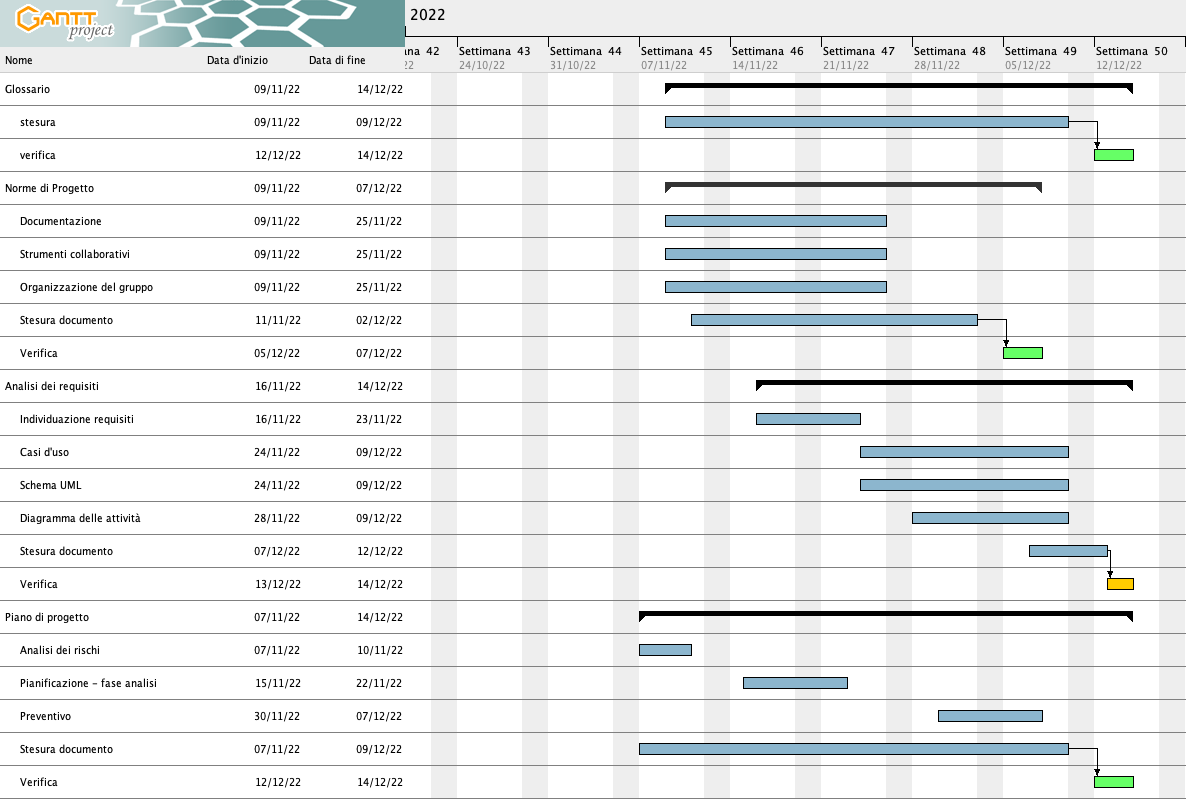
\includegraphics[scale=0.38]{image/analisi_preliminare_gantt.png}
    \caption{Diagramma di Gantt\textsubscript{g} fase di Analisi preliminare}
\end{figure}
\pagebreak
%fase PoC

\subsection{Progettazione Proof of Concept\textsubscript{g}}
Questo periodo comincia al termine del periodo di Analisi preliminare e termina con l'inizio della codifica del Proof of Concept\textsubscript{g}.\\
\begin{center}
\textbf{periodo:} dal 15-12-2022 al 16-01-2023\\
\end{center}
Questo periodo viene dedicato al completamento delle attività arretrate, per poi concentrarsi sulla 
progettazione e iniziare la codifica del Proof of Concept\textsubscript{g}. Si va inoltre avanti con la stesura 
della documentazione. Questo periodo viene suddiviso nelle attività trattate nella seguente sezione.

\subsubsection{Attività}
\begin{itemize}
\item \textbf{\textit{Glossario}:} il documento viene costantemente aggiornato con nuovi termini;
\item \textbf{\textit{Piano di Progetto}:} viene aggiunta la pianificazione del periodo, il preventivo e il consultivo;  
\item \textbf{Analisi dei requisti:} si continua la stesura del documento, completando le attività arretrate dal periodo precedente;
\item \textbf{\textit{Piano di Qualifica}:} documento nel quale vengono stabiliti gli standard di qualità di processo\textsubscript{g} e di prodotto\textsubscript{g};
\item \textbf{\textit{Norme di Progetto}:} vengono aggiunte nuove norme relative alla documentazione e alle metriche utilizzate nel \textit{Piano di Qualifica};
\item \textbf{Proof of Concept\textsubscript{g}:} ogni componente del gruppo studierà individualmente le tecnologie da utilizzare, per prendere familliarità; si inizierà poi a progettare e realizzare il Proof of Concept\textsubscript{g}, una versione semplice, ma dimostrativa, del prodotto\textsubscript{g} finale, per 
capire se è fattibile e darne una prova al proponente\textsubscript{g}.
\end{itemize}

\subsubsection{Periodi}
La Progettazione Proof of Concept\textsubscript{g} sarà suddivisa nei seguenti periodi:
\begin{itemize}
\item \textbf{Periodo 1:} \textit{dal 15-12-2022 al 21-12-2022}, pianificazione del periodo corrente con relativo preventivo, completamento attività arretrate 
(stesura del documento \textit{Analisi dei Requisiti}). Continua lo studio individuale delle tecnologie da utilizzare;
\item \textbf{Periodo 2:} \textit{dal 22-12-2022 al 04-01-2023}, inizia la stesura del documento \textit{Piano di Qualifica}. Inizia la progettazione del Proof of Concept\textsubscript{g}, si continua la stesura e la verifica\textsubscript{g} dei documenti;
\item \textbf{Periodo 3:} \textit{dal 05-01-2023 al 16-01-2023}, continua la progettazione e inizia la codifica del Proof of Concept\textsubscript{g}. Si procede nella stesura e nella verifica\textsubscript{g} della documentazione.
\end{itemize}

\begin{figure}[H]
    \centering
    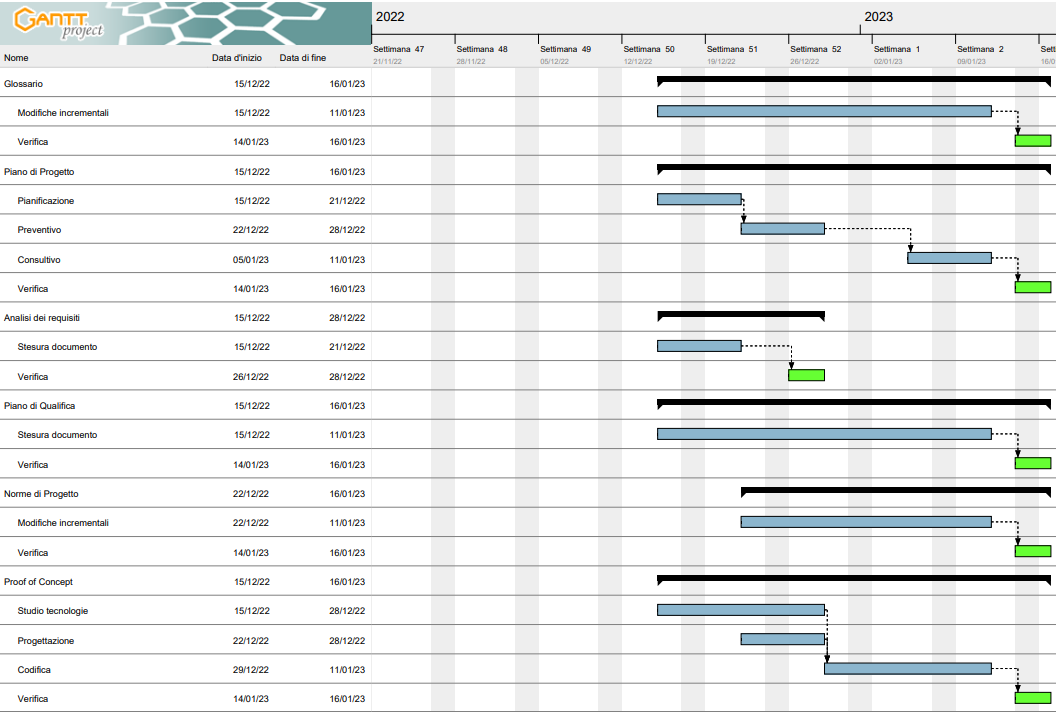
\includegraphics[scale=0.72]{image/gantt_poc.png}
    \caption{Diagramma di Gantt\textsubscript{g} fase di Progettazione Proof of Concept\textsubscript{g}}
\end{figure}
\pagebreak

\subsection{Codifica Proof of Concept\textsubscript{g}}
Questo periodo comincia al termine del periodo di Progettazione Proof of Concept\textsubscript{g} e termina con 
la consegna dei documenti per la Requirements and Tecnology Baseline.\\
\begin{center}
\textbf{periodo:} dal 17-01-2023 al 15-02-2023\\
\end{center}
In questo periodo ci si concentra sul portare a termine la codifica del Proof of Concept\textsubscript{g}, viene completata la stesura della documentazione, che 
viene alla fine approvata per la RTB. 

\subsubsection{Attività}
\begin{itemize}
\item \textbf{\textit{Glossario}:} il documento viene costantemente aggiornato con nuovi termini;
\item \textbf{\textit{Piano di Progetto}:} viene aggiunta la pianificazione del periodo, il preventivo e il consultivo;  
\item \textbf{Analisi dei Requisti:} si termina la stesura del documento applicando le modifiche necessarie;
\item \textbf{\textit{Piano di Qualifica}:} si continua con la stesura del documento;
\item \textbf{\textit{Norme di Progetto}:} viene cambiato l'indice del documento per avere una conformità con il \textit{Piano di Qualifica}, 
si completa la stesura delle sezioni mancanti;
\item \textbf{Proof of Concept\textsubscript{g}:} si completa la codifica del PoC\textsubscript{g}, aggiungendo le funzionalità stabilite in accordo con il proponente\textsubscript{g}.
\end{itemize}

\subsubsection{Periodi}
Il periodo di Codifica Proof of Concept\textsubscript{g} sarà suddivisa nei seguenti periodi:
\begin{itemize}
\item \textbf{Periodo 1:} \textit{dal 17-01-2023 al 31-01-2023}, pianificazione del periodo corrente con relativo preventivo, si continua la codifica 
del Proof of Concept\textsubscript{g}. Prosegue la stesura del \textit{Piano di Qualifica} aggiornando le metriche da seguire; si aggiornano le \textit{Norme di Progetto} di conseguenza;
\item \textbf{Periodo 2:} \textit{dal 01-02-2023 al 15-02-2023},  viene completata la codifica del PoC\textsubscript{g} e la stesura della documentazione. 
Si verifica\textsubscript{g} nel \textit{Piano di Qualifica} che le metriche siano rispettate. Si verificano e approvano tutti i documenti in previsione della RTB.
\end{itemize}

\begin{figure}[H]
    \centering
    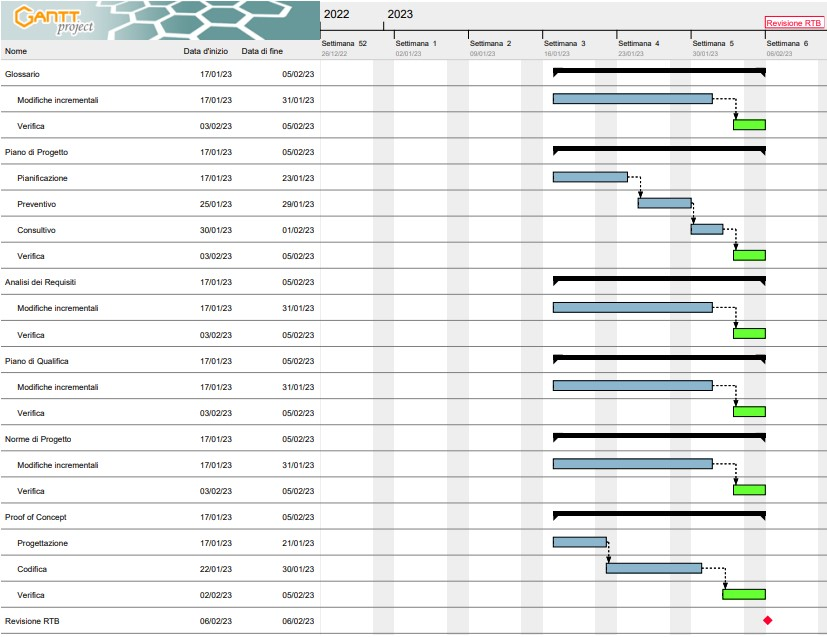
\includegraphics[scale=0.56]{image/gantt_terzo_periodo.png}
    \caption{Diagramma di Gantt\textsubscript{g} fase di Codifica Proof of Concept\textsubscript{g}}
\end{figure}
\pagebreak

\subsection{Progettazione di dettaglio e codifica dei requisiti}
Questo periodo inizia subito dopo la revisione di Requirements and Technology Baseline (RTB\textsubscript{g}) e si conclude con l'avvio della Validazione e Collaudo. Non procederemo con un aggiornamento diretto del nostro PoC\textsubscript{g}, ma piuttosto utilizzeremo il suo codice per creare una versione migliore utilizzando ulteriori librerie introdotte per facilitare l’implementazione dei pattern architetturali.
\begin{center}
\textbf{periodo:} dal 29-03-2023 al 03-05-2023\\
\end{center}
\subsubsection{Attività}
\begin{itemize}
\item \textbf{Documentazione:} vengono effettuate modifiche correttive ai documenti che necessitano di un aggiornamento o di una revisione;
\item \textbf{Codifica:} i programmatori creano il codice del prodotto basato sulle attività individuate all'inizio dello Sprint\textsubscript{g}, partendo dalla base del periodo precedente e aggiungendo nuove funzionalità per ottenere una versione funzionante del prodotto;
\item \textbf{Product Baseline\textsubscript{g}:} quest'attività introduce la baseline architetturale del prodotto attraverso i diagrammi delle classi e di sequenza, dimostrando la coerenza con quanto presentato durante l'attività di Technology Baseline;  
\item \textbf{Test:} i programmatori creano test di unità e di integrazione per i componenti sviluppati durante questo periodo;
\item \textbf{Manuali:} vengono redatti il \textit{Manuale Utente} e \textit{Manuale Sviluppatore}, in relazione alle funzionalità implementate. Questi documenti forniscono istruzioni sull'uso del sistema per gli utenti coinvolti.
\end{itemize}

\subsubsection{Backlog}
In questa sezione è riportata la tabella del backlog, così strutturata:
\begin{itemize}
    \item \textbf{Task:} il nome della task;
    \item \textbf{Descrizione:} una breve descrizione della task;
    \item \textbf{Data inizio:} la data in cui si pianifica di iniziare la task, oppure viene indicato con "-" che la task in 
    questione è ricorrente;
    \item \textbf{Attività:} l'attività a cui fa riferimento la task. Le attività possono essere: PB, (Product Baseline), Doc (Documentazione), Test o Manuali.
\end{itemize}
\begin{longtable}{ 
	>{\centering}M{0.23\textwidth} 
	>{\centering}M{0.44\textwidth}
	>{\centering}M{0.13\textwidth}
	>{\centering}M{0.10\textwidth}
	}
	\rowcolorhead
	\centering 
	\headertitle{Task} &	
	\headertitle{Descrizione} &
	\headertitle{Data inizio} &
	\headertitle{Attività}
	\endfirsthead	
	\endhead
	
	Apprendimento librerie & Si studiano individualmente le librerie scelte & 29-03-2023 & PB \tabularnewline
	Individuazione pattern architetturali & Si individuano dei pattern architetturali adeguati & 29-03-2023 & PB \tabularnewline
	Diagramma delle classi & Viene prodotto il diagramma delle classi & 07-04-2023 & PB \tabularnewline
	Diagramma di sequenza & Viene prodotto il diagramma di sequenza & 10-04-2023 & PB \tabularnewline
	Correzione Piano di Qualifica & Viene sistemato il Piano di Qualifica in base alle correzioni nella RTB & 29-03-2023 & Doc \tabularnewline
	Aggiornamento grafici Piano di Qualifica & Vengono calcolati i valori delle metriche e aggiornati i grafici & 05-04-2023 & Doc \tabularnewline
	Modello di sviluppo nel Piano di Progetto & Viene cambiato il modello di sviluppo, passando al modello agile & 29-03-2023 & Doc \tabularnewline
	Pianificazione sprint nel Piano di Progetto & Viene pianificato lo sprint successivo & - & Doc \tabularnewline
	Preventivo dello sprint nel Piano di Progetto & Viene calcolato il preventivo per lo sprint successivo & - & Doc \tabularnewline
	Consuntivo dello sprint nel Piano di Progetto & Viene calcolato il consuntivo per lo sprint concluso & - & Doc \tabularnewline
	Diario di Bordo & Viene scritto il Diario di Bordo & - & Doc \tabularnewline
	Verbale & Viene redatto il verbale al termine di ogni riunione & - & Doc \tabularnewline
	Correzione Norme di Progetto & Vengono sistemate le Norme di Progetto in base alle correzioni nella RTB & 29-03-2023 & Doc \tabularnewline
	Aggiornamento Norme di Progetto & Vengono aggiunte le norme sulla codifica & 12-04-2023 & Doc \tabularnewline
	Specifica Tecnica & Viene scritto il documento \textit{Specifica Tecnica} & 14-04-2023 & Doc \tabularnewline
	Manuale Utente & Viene scritto il documento \textit{Manuale Utente} & 21-04-2023 & Manuali \tabularnewline
	Manuale Sviluppatore & Viene scritto il documento \textit{Manuale Sviluppatore} & 21-04-2023 & Manuali \tabularnewline
	Test di unità & Vengono scritti i test di unità & - & Test \tabularnewline
	Test di integrità & Vengono scritti i test di integrità & - & Test \tabularnewline
	Test di sistema & Vengono scritti i test di sistema & - & Test \tabularnewline
	Test di accettazione & Vengono scritti i test di accettazione & - & Test \tabularnewline
	\captionline \caption{Backlog: Progettazione di dettaglio e codifica dei requisiti}
\end{longtable}

\subsubsection{Sprint 2}
\begin{center}
\textbf{periodo:} dal 06-04-2023 al 13-04-2023\\
\end{center}
In questo sprint\textsubscript{g} il gruppo si concentra a produrre un possibile diagramma delle classi. 
Nel caso avanzino ore lavorative ci occuperemo della produzione di un possibile diagramma di sequenza e di iniziare la stesura delle norme
di codifica.

Attualmente le task presenti nel backlog sono le seguenti:

\begin{longtable}{ 
	>{\centering}M{0.23\textwidth} 
	>{\centering}M{0.44\textwidth}
	>{\centering}M{0.13\textwidth}
	>{\centering}M{0.10\textwidth}
	}
	\rowcolorhead
	\centering 
	\headertitle{Task} &	
	\headertitle{Descrizione} &
	\headertitle{Data inizio} &
	\headertitle{Attività}
	\endfirsthead	
	\endhead
	
	Diagramma delle classi & Viene prodotto il diagramma delle classi & 06-04-2023 & PB \tabularnewline
	Verbale del VI\_06-04-2023 & Viene redatto il verbale  VI\_06-04-2023& 06-04-2023 & Doc \tabularnewline
	Verbale del VE\_05-04-2023 & Viene redatto il verbale VE\_05-04-2023& 06-04-2023 & Doc \tabularnewline
	Diario di Bordo del 10-04-2023 & Viene scritto il Diario di Bordo del 10-04-2023 & 09-04-2023 & Doc \tabularnewline
	Pianificazione sprint 3 & Viene pianificato lo sprint 3 & 11-04-2023 & Doc \tabularnewline
	Diagramma di sequenza & Viene prodotto il diagramma di sequenza & 10-04-2023 & PB \tabularnewline
	Norme sulla codifica & Vengono aggiunte le norme sulla codifica & 10-04-2023 & Doc \tabularnewline
	Norme sui test di unità & Vengono scritte le norme sui test di unità & - & Test \tabularnewline
	Norme sui test di integrità & Vengono scritte le norme sui test di integrità & - & Doc \tabularnewline
	Norme sui test di sistema & Vengono scritte le norme sui test di sistema & - & Doc \tabularnewline
	Norme sui test di accettazione & Vengono scritte le norme sui test di accettazione & - & Doc \tabularnewline
	Specifica Tecnica & Viene scritto il documento \textit{Specifica Tecnica} & - & Doc \tabularnewline
	Manuale Utente & Viene scritto il documento \textit{Manuale Utente} & - & Doc \tabularnewline
	Manuale Sviluppatore & Viene scritto il documento \textit{Manuale Sviluppatore} & - & Doc \tabularnewline
	\captionline \caption{Backlog: Progettazione di dettaglio e codifica dei requisiti}
\end{longtable}

Le task assegnate per questo sprint sono:
\begin{longtable}{ 
	>{\centering}M{0.30\textwidth} 
	>{\centering}M{0.10\textwidth}
	}
	\rowcolorhead
	\centering 
	\headertitle{Task} &	
	\headertitle{Priorità}
	\endfirsthead	
	\endhead
	
	Diagramma delle classi & Alta \tabularnewline
	Diario di Bordo del 10-04-2023 & Alta \tabularnewline
	Verbale del VI\_06-04-2023 & Alta \tabularnewline
	Verbale del VE\_05-04-2023 & Alta \tabularnewline
	Pianificazione sprint 3 & Alta \tabularnewline
	Diagramma di sequenza & Media \tabularnewline
	Norme sulla codifica & Media \tabularnewline
	
\end{longtable}

\begin{figure}[H]
	\centering 
	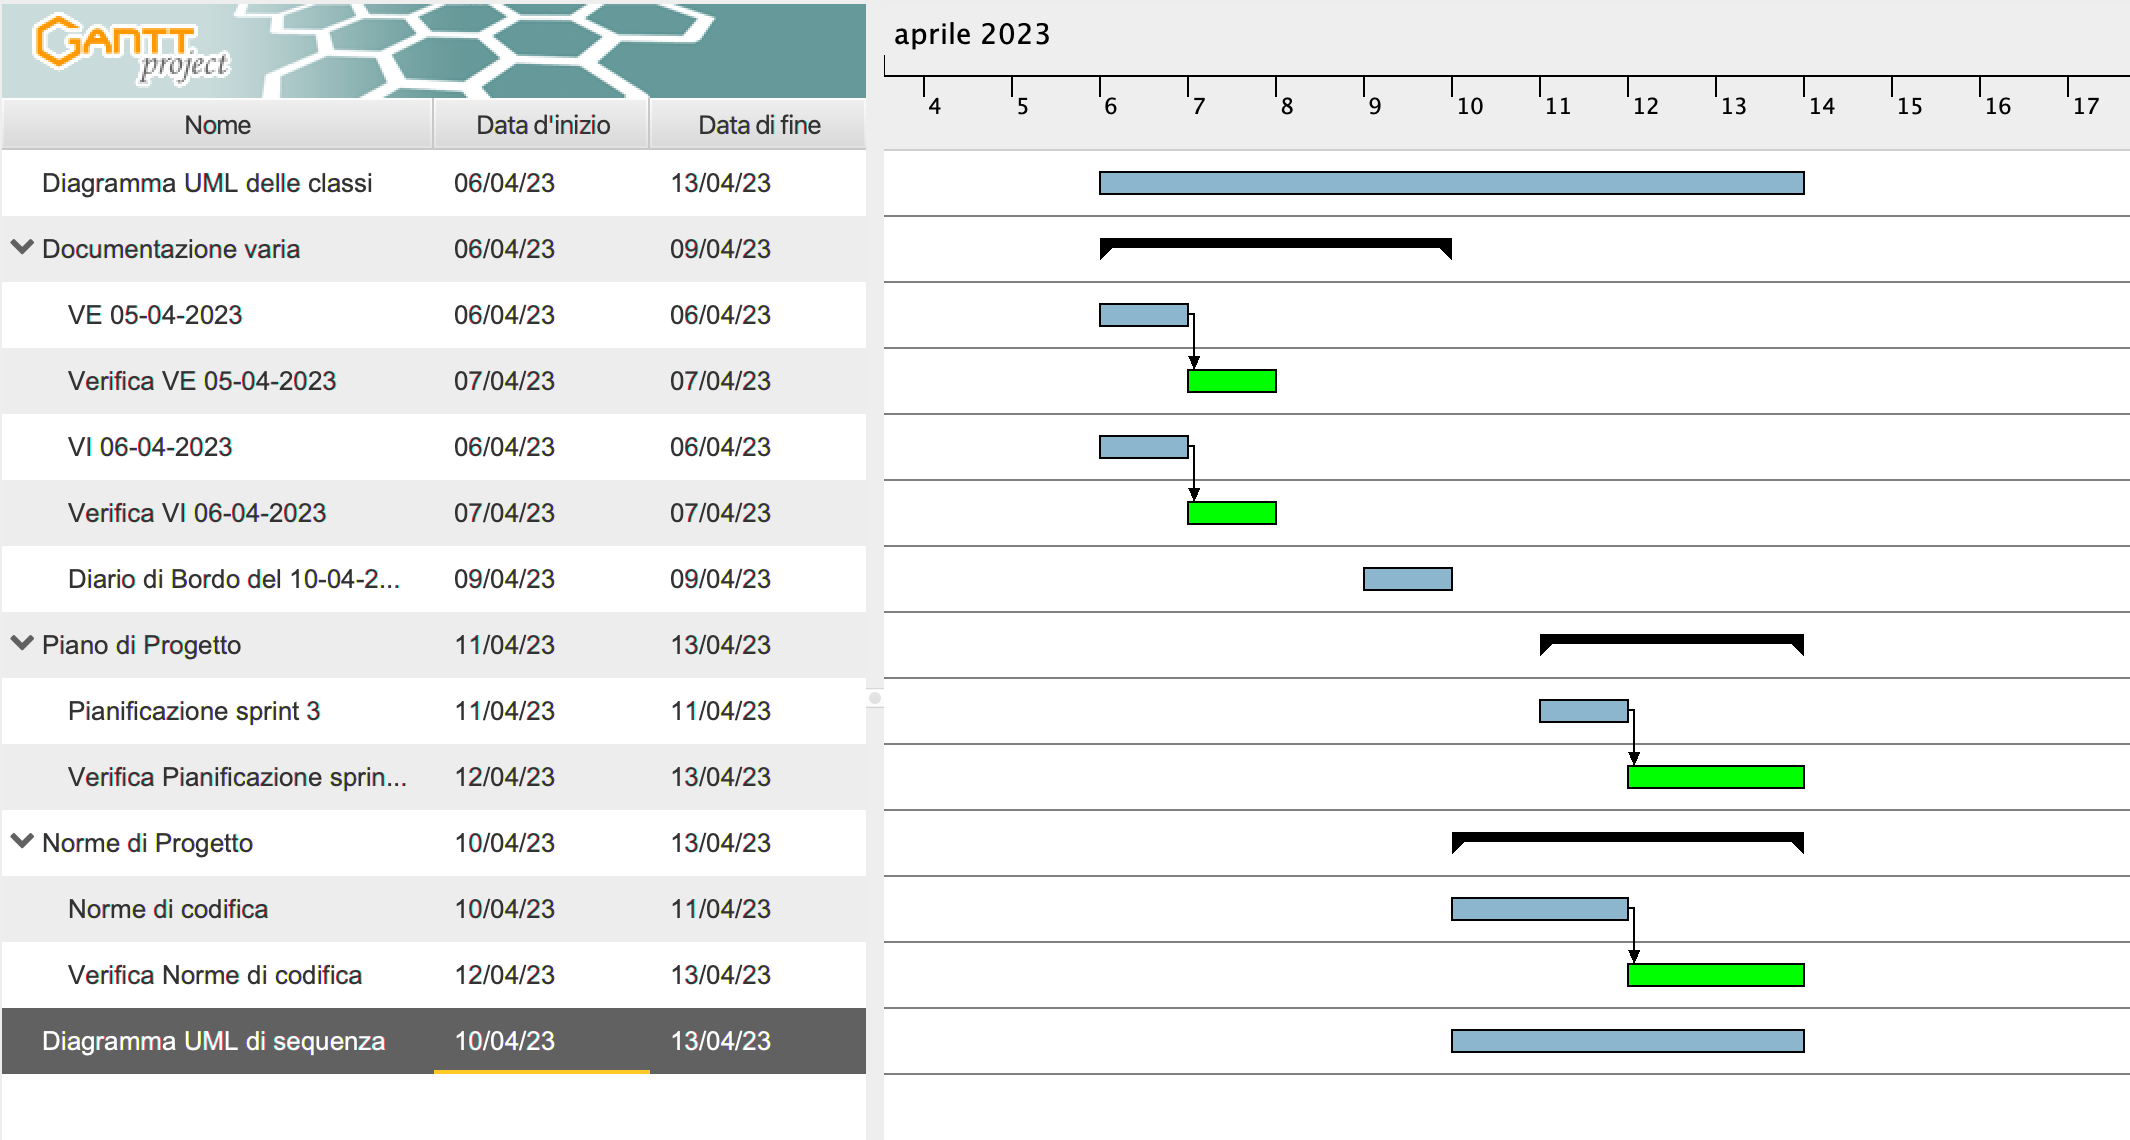
\includegraphics[scale=0.42]{image/gantt_sprint2.PNG}
	\caption{Diagramma di Gantt\textsubscript{g} Sprint\textsubscript{g} 2}
\end{figure}
\pagebreak